Antes de comenzar con las búsquedas propuestas se debe definir una función de similitud entre los 
elementos pertenecientes al conjunto de búsqueda y una noción de complementariedad entre ellos.\\
Una vez definido estos parámetros de comparación se puede comenzar con la generación de bundles que 
luego algunos de ellos formarán parte de la solución entregada.
%\\
%Para los siguientes búsquedas asumamos que tenemos el siguiente conjunto de papers.\\ \\
%Conferencia \textbf{SIGSOFT FSE}
\begin{itemize}
  \begin{small}
  \item Experience report: using RESOLVE/C++ for commercial software.\\
  Bruce W. Weide (Ohio State University), Joseph E. Hollingsworth (Indiana University Southeast), Lori Blankenship (Holly Software, Inc. Floyds Knobs).\\
  $0.25\%$ LANGUAGES, $0.25\%$ KNOWLEDGE ENGINEERING, $0.50\%$ FORMAL METHODS.
  \item Interpolation for data structures.\\
  Rupak Majumdar (University of California Los Angeles), Deepak Kapur (University of New Mexico), Calogero G. Zarba (Saarland University).\\
  $0.50\%$ LANGUAGES, $0.50\%$ FORMAL METHODS.
  \item An empirical study of the effect of time constraints on the cost-benefits of regression testing.\\
  Gregg Rothermel (University of Nebraska Lincoln), Hyunsook Do (North Dakota State University), Siavash Mirarab (University of Waterloo), Ladan Tahvildari (University of Waterloo).\\
  $0.33\%$ TESTING, $0.67\%$ RELIABILITY.
  \item Differential symbolic execution.\\
  Sebastian G. Elbaum (University of Nebraska Lincoln), Matthew B. Dwyer (University of Nebraska Lincoln), Corina S. Pasareanu (National Aeronautics and Space, Administration, United States), Suzette Person (National Aeronautics and Space Administration, United States).\\
  $0.25\%$ TESTING, $0.25\%$ ARCHITECTURES, $0.50\%$ FORMAL METHODS.
  \end{small}
\end{itemize}

Conferencia \textbf{ASE}
\begin{itemize}
  \begin{small}
  \item The power of software.\\
  Alfonso Fuggetta (Politecnico di Milano). \\
  $0.75\%$ LANGUAGES, $0.25\%$ SOFTWARE QUALITY.
  \item Bogor/Kiasan: A k-bounded Symbolic Execution for Checking Strong Heap Properties of Open Systems.\\
  Xianghua Deng (Pennsylvania State University), Jooyong Lee (Korea University), Robby (Kansas State University).\\
  $0.30\%$ TESTING, $0.30\%$ LANGUAGES, $0.40\%$ FORMAL METHODS.
  \item A dynamic birthmark for java.\\
  Christian Lindig (Harvard University), David Schuler (Saarland University), Valentin Dallmeier (Saarland University).\\
  $0.67\%$ TESTING, $0.33\%$ SECURITY.
  \item MTSA: The Modal Transition System Analyser.\\
  Marsha Chechik (University of Toronto), Sebastián Uchitel (Universidad de Buenos Aires), Nicolás D'Ippolito (Universidad de Buenos Aires), Dario Fischbein (Imperial College London).\\
  $0.625\%$ MODELS, $0.375\%$ FORMAL METHODS.
  \end{small}
\end{itemize}

Conferencia \textbf{ICSE}
\begin{itemize}
  \begin{small}
  \item Modeling ontologies as executable domain specific languages.\\
  Dragan Djuric (NULL), Jelena Jovanovic (University of Belgrade), Ramo Sendelj (Mediterranean University Montenegro), Vladan Devedzic (University of Belgrade).\\
  $0.50\%$ TESTING, $0.50\%$ DISTRIBUTED SYSTEMS.
  \item The Property Vector Specification of a Multiset Iterator.\\
  David Alex Lamb (Liverpool John Moores University), Trevor W. Pearce (Carleton University).\\
  $0.67\%$ LANGUAGES, $0.25\%$ FORMAL METHODS.
  \item Modeling behavioral design patterns of concurrent objects.\\
  Hassan Gomaa (George Mason University), Robert G. Pettit IV (George Mason University).\\
  $0.50\%$ LANGUAGES, $0.50\%$ DISTRIBUTED SYSTEMS.
  \item How we refactor, and how we know it.\\
  Andrew P. Black (Portland State University), Chris Parnin (Georgia Institute of Technology), Emerson R. Murphy-Hill (North Carolina State University).\\
  $0.33\%$ LANGUAGES, $0.67\%$ PROGRAM COMPREHENSION.
  \end{small}
\end{itemize}

Conferencia \textbf{ACM Trans. Softw. Eng. Methodol.}
\begin{itemize}
  \begin{small}
  \item A Time-Sensitive Object Model for Real-Time Systems.\\
  H. Rebecca Callison (University of Washington).\\
  $0.33\%$ REAL TIME SYSTEMS, $0.33\%$ LANGUAGES, $0.34\%$ FORMAL METHODS.
  \item Distributed Real-Time System Specification and Verification in APTL.\\
  Aloysius K. Mok (University of Texas Austin), Farn Wang (National Taiwan University), E. Allen Emerson (University of Texas Austin).\\
  $0.33\%$ LANGUAGES, $0.33\%$ DISTRIBUTED SYSTEMS, $0.34\%$ FORMAL METHODS.
  \item The role of outcome feedback in improving the uncertainty assessment of software development effort estimates.\\
  Magne Jørgensen (Simula Research Laboratory), Tanja M. Gruschke (Simula Research Laboratory).\\
  $0.50\%$ MAINTENANCE, $0.50\%$ INFORMATION SYSTMS.
  \item An inheritance-based technique for building simulation proofs incrementally.\\
  Nancy A. Lynch (Massachusetts Institute of Technology), Idit Keidar (Technion Israel Institute of Technology), Roger Khazan (Massachusetts Institute of Technology), Alexander A. Shvartsman (University of Connecticut).\\
  $0.50\%$ LANGUAGES, $0.50\%$ DISTRIBUTED SYSTEMS.
  \end{small}
\end{itemize}

Conferencia \textbf{IEEE Trans. Software Eng.}
\begin{itemize}
  \begin{small}
  \item An Empirical Study of Test Case Filtering Techniques Based on Exercising Information Flows.\\
  Wes Masri (American University of Beirut), David Leon (Case Western Reserve University), Andy Podgurski (Case Western Reserve University).\\
  $0.26\%$ TESTING, $0.14\%$ LANGUAGES, $0.60\%$ RELIABILITY.
  \item Synthesis of Decision-Free Concurrent Systems for Prescribed Resources and Performance.\\
  Tadao Murata (University of Illinois Chicago).\\
  $0.25\%$ DISTRIBUTED SYSTEMS, $0.75\%$ FORMAL METHODS.
  \item Independent Recovery in Large-Scale Distributed Systems.\\
  Peter Triantafillou (University of Patras).\\
  $0.33\%$ DATABASE, $0.33\%$ DISTRIBUTED SYSTEMS, $0.34\%$ KNOWLEDGE ENGINEERING.
  \item On Parallel Processing Systems: Amdahl's Law Generalized and Some Results on Optimal Design.\\
  Leonard Kleinrock (University of California Los Angeles), Jau-Hsiung Huang (National Taiwan University).\\
  $0.67\%$ DISTRIBUTED SYSTEMS, $0.33\%$ RELIABILITY.
  \end{small}
\end{itemize}
\section{similitud entre elementos}
En todas las búsquedas para poder definir la similitud entre elementos, partimos de los perfiles de los papers que pueden ser vistos como vectores de $N$ dimensiones normalizados ya que cada compenente representa un porcentaje del tema al que hace referencia.\\
Con estos vectores podemos calcular el ángulo que forman entre sí uno a uno y a partir de ese ángulo decidir su similitud, porque dos vectores que forman un ángulo cercano a $0$ nos representa que son muy similares.\\
\subsection{Cálculo de ángulos}
Para los siguientes cálculos mostramos en $\Re^{2}$ por ser visualmente más fácil de exponer, pero es todo extensible a $\Re^{n}$.\\
Recordemos el cálculo de un ángulo para dos vectores $V, U$:\\
$$\cos(\hat{\theta}) = \dfrac{\overrightarrow{V}.\overrightarrow{U}}{\overrightarrow{\lVert V\lVert}.\overrightarrow{\lVert U\lVert}}$$
A continuación podemos ver como se comporta la función $\cos$\\
\begin{figure}[H]
  \centering
    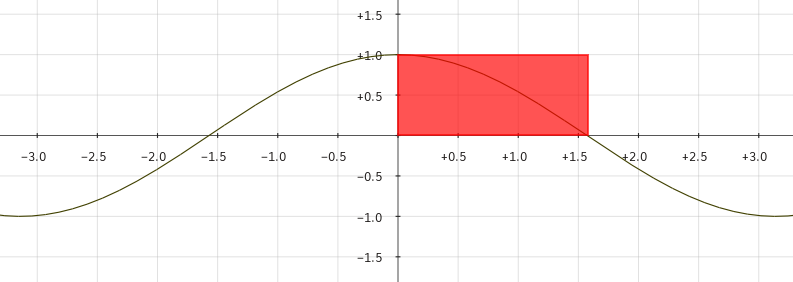
\includegraphics[width=0.8\textwidth]{img/coseno.png}
  \caption{Comportamiento de la función $\cos$. En rojo la región que involucra nustros resutlados}
  \label{bus:img-coseno}
\end{figure}
Si bien la función es circular, en nuestro problema particular solo nos centramos en un área de ella, ya que nuestros vectores solo pertenecen a un solo cuadrante del plano y además estan normalizados porque son porcentajes, con lo cuál sus componentes siempre serán positivas.\\
\begin{figure}[H]
  \centering
    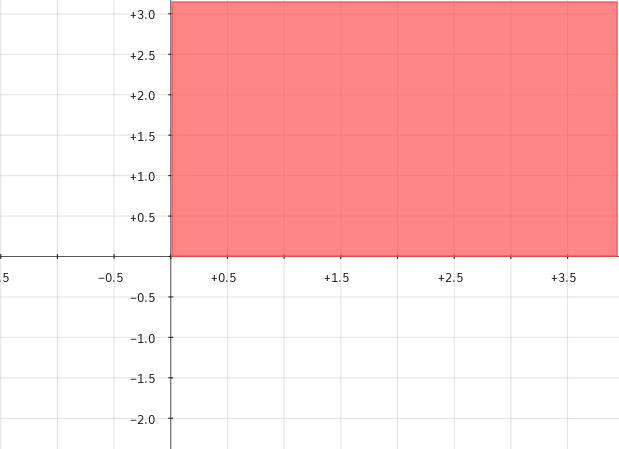
\includegraphics[width=0.4\textwidth]{img/planoCartesiano.png}
  \caption{Plano cartesiano. En rojo al cuadrante al que pertenecen nuestros vectores}
  \label{bus:img-planoCartesiano}
\end{figure}
De la anterior imágen podemos concluir que los ángulos que podemos obtener se encuentran limitados entre $0 \textdegree$ y $90 \textdegree$, o lo que es lo mismo $0$ y $\frac{\pi}{2}$. De todo lo anterior obtenemos que:
$$0\leq \cos(\hat{\theta}) \leq 1$$
Como en la región que nos interesa la función $\cos$ es decreciente y su inversa $\arccos$ también lo es en el intervalo deseado $[0, 1]$. Entonces buscar el menor ángluo $\theta$ o su $\cos$ nos resulta similar. Con lo cuál decidimos siempre buscar el $\cos(\theta)$.\\
Siempre que dos vectores tengan un ángulo cercano a $0$ más similares van a ser los papers. Eso lo podemos ver geometricamente cuando dos vectores tienen un ángulo igual a $0$ quiere decir que son paralelos o en nuestro problema particular son iguales ya que están todos normalizados y ángulos cercano a $90 \textdegree$ es porque son ortogonales y no tienen ningún atributo en común por lo que no son en nada similares.
\section{Papers similares, diferentes conferencias}\label{bus:papSimDisLug}
El objetivo de esta búsqueda es generar una solución de bundles, en el que cada elemento contenga 
papers de tópicos similares pero que se hayan presentado en distintas conferencias.\\
Para realizar esta búsqueda se debe definir que se entiende por papers de tópicos similares y cual 
es la presentación de la conferencia. Para ello en la base de datos \cite{dataDrive} cuenta 
con la información de la presentación del paper, \texttt{venue} de ahora en adelante, y los 
perfiles de cada paper, \texttt{topicProfile} a partir de ahora.\\
La primer característica se utilizó para la complementariedad de dos papers, por lo que en cada 
bundle no habrá dos papes de un mismo \texttt{venue}. Cada paper se representó
con un vector de dimensión $N$ en el que el valor de cada elemento es el porcentaje del \texttt{topicProfile}.\\ 
La función de similitud se define como la distancia angular entre los vectores.
%\\
%Si tomamos nuestro universo de ejemplo y decidimos buscar 3 bundles de 2 elementos, esperaríamos obtener el siguiente resutlado:
%\begin{small}
  \begin{itemize}
    \item Bundle 1
    \begin{itemize}
      \item Synthesis of Decision-Free Concurrent Systems for Prescribed Resources and Performance.\\
      Tadao Murata (University of Illinois Chicago).\\
      $0.25\%$ DISTRIBUTED SYSTEMS, $0.75\%$ FORMAL METHODS.
      \item Differential symbolic execution.\\
      Sebastian G. Elbaum (University of Nebraska Lincoln), Matthew B. Dwyer (University of Nebraska Lincoln), Corina S. Pasareanu (National Aeronautics and Space, Administration, United States), Suzette Person (National Aeronautics and Space Administration, United States).\\
      $0.25\%$ TESTING, $0.25\%$ ARCHITECTURES, $0.50\%$ FORMAL METHODS.
    \end{itemize}
    \item Bundle 2
    \begin{itemize}
      \item An empirical study of the effect of time constraints on the cost-benefits of regression testing.\\
      Gregg Rothermel (University of Nebraska Lincoln), Hyunsook Do (North Dakota State University), Siavash Mirarab (University of Waterloo), Ladan Tahvildari (University of Waterloo).\\
      $0.33\%$ TESTING, $0.67\%$ RELIABILITY.
      \item An Empirical Study of Test Case Filtering Techniques Based on Exercising Information Flows.\\
      Wes Masri (American University of Beirut), David Leon (Case Western Reserve University), Andy Podgurski (Case Western Reserve University).\\
      $0.26\%$ TESTING, $0.14\%$ LANGUAGES, $0.60\%$ RELIABILITY.
    \end{itemize}
    \item Bundle 3
    \begin{itemize}
      \item The power of software.\\
      Alfonso Fuggetta (Politecnico di Milano). \\
      $0.75\%$ LANGUAGES, $0.25\%$ SOFTWARE QUALITY.
      \item The Property Vector Specification of a Multiset Iterator.\\
      David Alex Lamb (Liverpool John Moores University), Trevor W. Pearce (Carleton University).\\
      $0.67\%$ LANGUAGES, $0.25\%$ FORMAL METHODS.
    \end{itemize}
  \end{itemize}
\end{small}
\section{Autores similares, distintas universidades}
Esta búsqueda consiste en encontrar una solución de bundles en el que cada bundle contiene autores 
similares pero de distinta universidad de afiliación.\\
Para determinar la similitud entre los autores se creó un perfil de cada uno. Para lograrlo lo 
primero que se hizo fue tener en cuenta todos los perfiles de papers en los que participaron cada 
uno de ellos. Al igual que con los papers, el perfil de los autores se representó con un vector. 
Este vector se cálculo sumarizando los vectores de cada uno de los papers en el que participó.\\
Para la función de similitud se utilizaron dos definiciones. La primera, al igual que con los papers,
consiste en la distancia angular. La otra definición es calcular la norma del vector resultante de la resta
vectorial entre los vectores de cada autor.\\
La complementariedad de dos papers se definió al lugar de pertenencia del autor en cuestión.
\section{Papers similares, con un perfil específico}
A la búsqueda de ``papers similares de diferente conferencia'' se le agregó una variante para ponderar
soluciones que contengan \texttt{topicProfile} específicos.
Para ello se agregó un parámetro que con el porcentaje de cada \texttt{topicProfile} para la ponderación.
Encontrar una solución de bundles de manera similar a ~\ref{bus:papSimDisLug} teniendo en cuenta que cada 
bundle además de compartir sus similitudes, también deben guardar relación con los tópicos 
específicos.\\
\section{Instituciones similares, diferentes regiones}
En este caso, la búsqueda es para instituciones similares de diferentes regiones. Al igual que con las 
búsquedas de autores, el perfil de cada institución se determino a partir del \texttt{topicProfile} de los papers
de estas. La complementariedad por la el atributo de la región de la institución. 
Luego el procedimiento para buscar soluciones, fue idéntico al utilizado para el de los autores.